\documentclass{article}
\usepackage[utf8]{inputenc}
\usepackage[spanish]{babel}
\usepackage{listings}
\usepackage{graphicx}
\graphicspath{ {images/} }
\usepackage{cite}

\begin{document}

\begin{titlepage}
    \begin{center}
        \vspace*{1cm}
            
        \Huge
        \textbf{LA MEMORIA DEL COMPUTADOR}
            
        \vspace{0.5cm}
        \LARGE
        Un recurso informático invaluable.
        \vspace{1.5cm}
            
        \textbf{Julian Guillermo Zapata Rugeles}
            
        \vfill
            
        \vspace{0.8cm}
            
        \Large
        Despartamento de Ingeniería Electrónica y Telecomunicaciones\\
        Universidad de Antioquia\\
        Medellín\\
        Septiembre de 2020
            
    \end{center}
\end{titlepage}

\tableofcontents

\section{Qué es la memoria de un computador}
Para conocer qué es la memoria de un computador debemos preguntarnos cómo funciona, un ejemplo práctico es imaginarnos un pequeño recipiente que es capaz de almacenar una carga eléctrica por un breve periodo de tiempo. El comportamiento físico de nuestro 'recipiente' que en electrónica se llama condensador(pues es capaz de almacenar energía sustentando un campo eléctrico) nos permite representar dos estados. Cuando nuestro recipiente está lleno (un nivel máximo de electrones) y cuando está vacío (ausencia de un mínimo de electrones), sin embargo esto no es suficiente para darnos una idea clara de como funciona la memoria.
Para entender este nuevo concepto es necesario bajar en las capas de abstracción para imaginar que nuestros recipientes pueden agruparse en bloques, supongamos unos 8 recipientes por bloque (a este bloque lo llamaremos byte) y estos pueden tener algún estado de los expuestos anteriormente. Eso significa que podemos tener 2 posibles estados elevado a la octava potencia (pues tenemos 8 recipientes).


\begin{figure}[h]
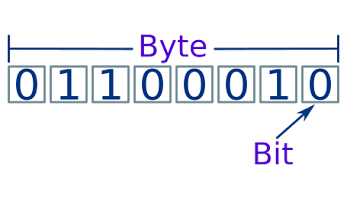
\includegraphics[width=4cm]{images/byte.png}
\centering
\caption{8 bits (8 recipientes)  agrupados en un bloque llamado byte. fuente imagen https://terminosaudiovisuales.es/byte/}
\label{fig:byte}
\end{figure}
\[2^{8}=256 \]
De manera abstracta podemos pensar en que cada número entre los 256 que se pueden obtener tras combinar los dos estados. Pueden representar 
 análogamente una letra, número o símbolo de nuestro alfabeto. La disposición de millones de bloques de nuestros recipientes pueden almacenar muchísimas representaciones abstractas de nuestro vocabulario y más.
Inmediatamente nos surge una pregunta qué a veces puede dejarnos perplejos , ¿cómo podemos incrustar millónes
 de estos componentes en una placa que tiene un tamaño similar a su dedo indice?. Si bien no profundizaré en las técnicas de grabado de estos circuitos si podemos formular una idea más puntual sobre que es la memoria, en síntesis nos permite almacenar la información que será procesada por el microcontrolador del computador, dada sus características físicas permite algunas mejoras sustanciales  
respecto a la velocidad de acceso y notorias ventajas como un sitio donde se puede almacenar / eliminar / mover y cambiar la información que será dispuesta por el procesador. Más adelante veremos que la memoria de un computador cumple con una organización jerárquica donde la capa superior están  
más próxima al procesador y el coste/bit aumenta significativamente. A medida que disminuimos en la jerarquía la cantidad de almacenamiento aumenta drásticamente pero su coste/bit disminuye
.\newline 

\section{Tipos de memoria}


La memoria de la computadora se caracteriza por tener múltiples prestaciones, cada una de ella tiene diferente clasificaciones / costes y funciones. Podemos sintetizar algunas de ellas en los principales grupos a continuación.\newline 

\subsection{Memoria de acceso secuencial}
Se caracteriza por tener bloques de datos llamados registros, dichos registros son secuenciales y para ser accedidos se debe pasar por cada uno de ellos hasta llegar al destino, naturalmente el tiempo que tardará en accederse a un registro es variable y depende de la posición.

    \begin{figure}[h]
    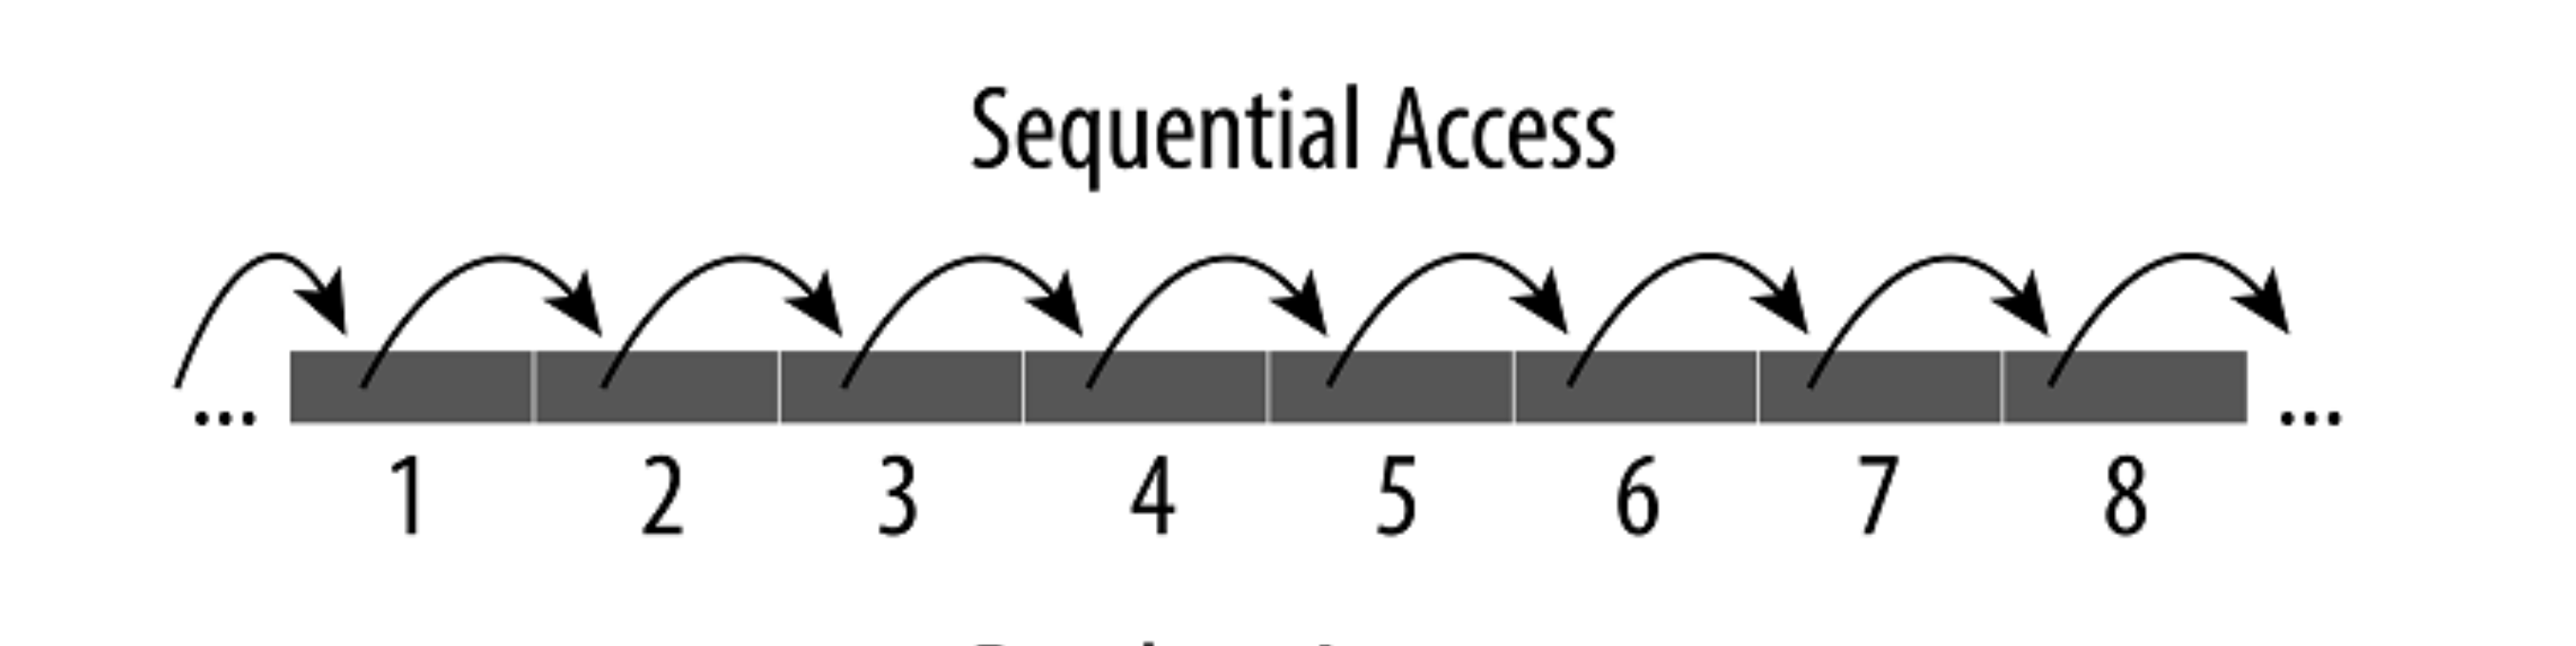
\includegraphics[width=6cm]{images/secuencial.png}
    \centering
    \label{fig:aleatory}
    \caption{Acceso secuencial}
    \end{figure}

\subsection{Memoria de acceso aleatorio} Cada posición de memoria está organizada de tal manera que posee un único mecanismos físico de acceso, por lo que a diferencia del secuencial podemos acceder a registros de forma independiente. Esto permite eliminar el tiempo variable y acceder con el mismo coste cualquier registro independiente de su posición.
 \label{aleatory}
    \begin{figure}[h]
    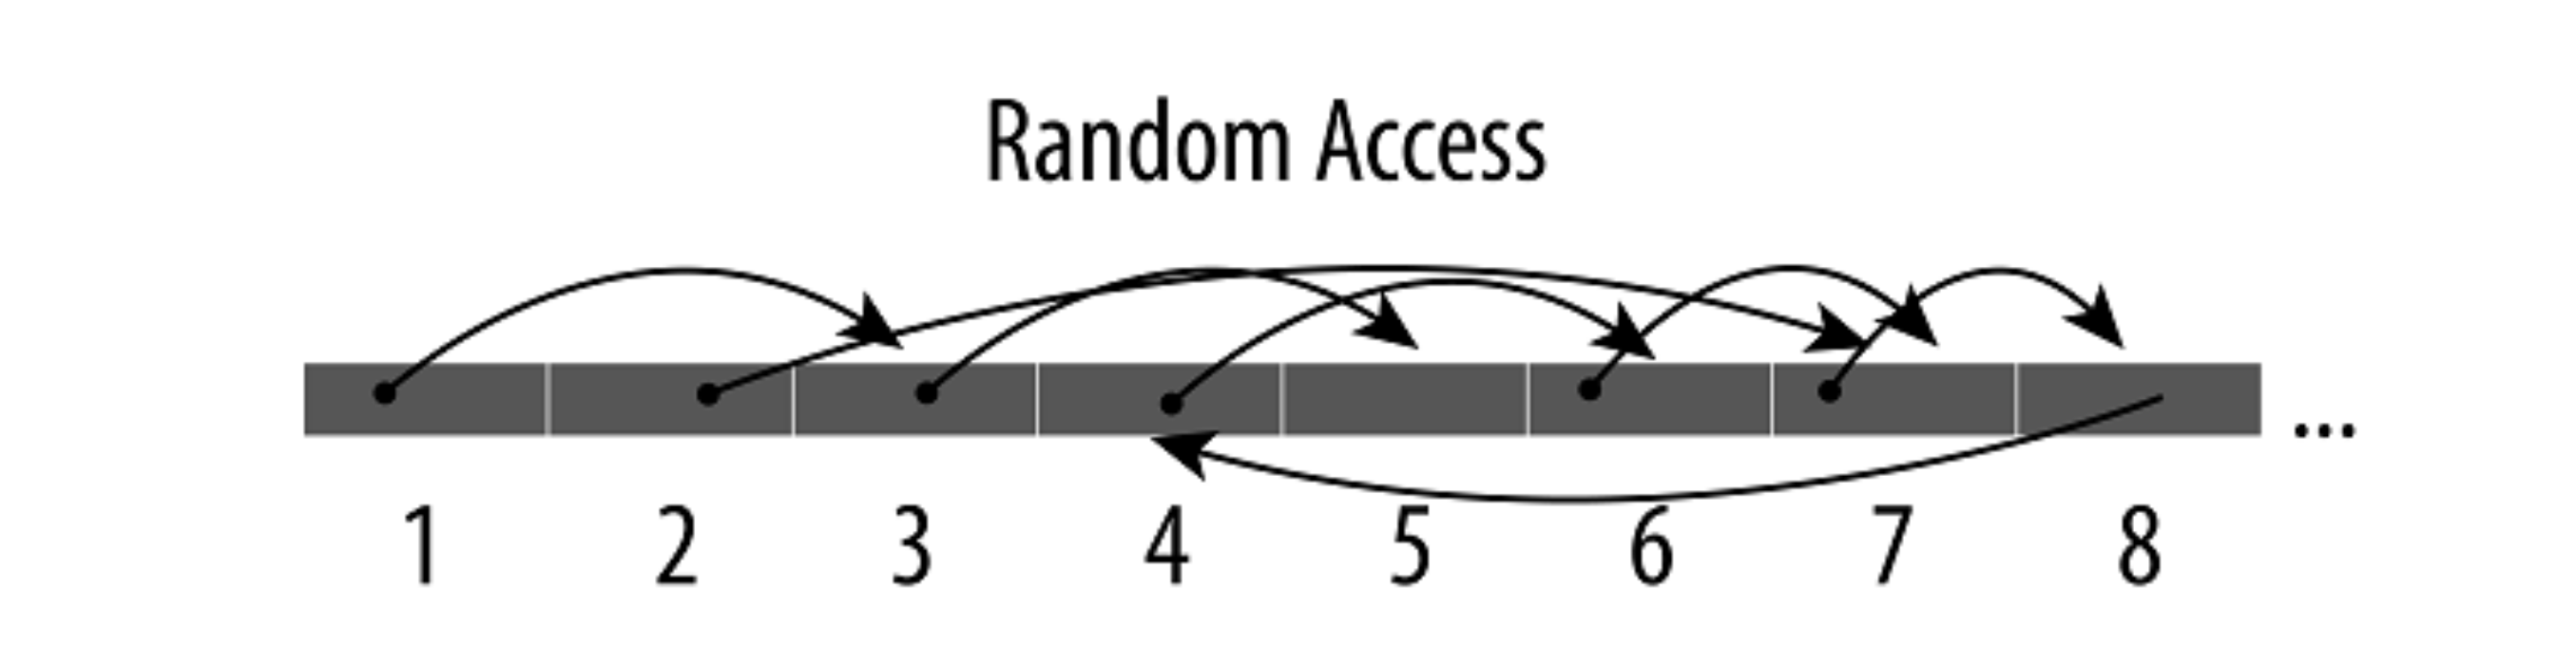
\includegraphics[width=6cm]{images/aleatorio.png}
    \centering
    \label{fig:aleatory}
    \caption{Acceso aleatorio}
    \end{figure}

\subsection{Memoria de acceso asociativo}
Este tipo de memoria conserva algunas características del tipo aleatorio. Además es capaz de hacer comparaciones de bits parciales teniendo parte del contenido a buscar en memoria, es por tanto una recuperación basada en porciones. Al igual que la memoria aleatoria tiene su mecanismo de direccionamiento y su tiempo de recuperación es constante.
Un ejemplo de ella es la\textbf{memoria caché}

\subsection{La memoria caché}
    \begin{figure}[h]
    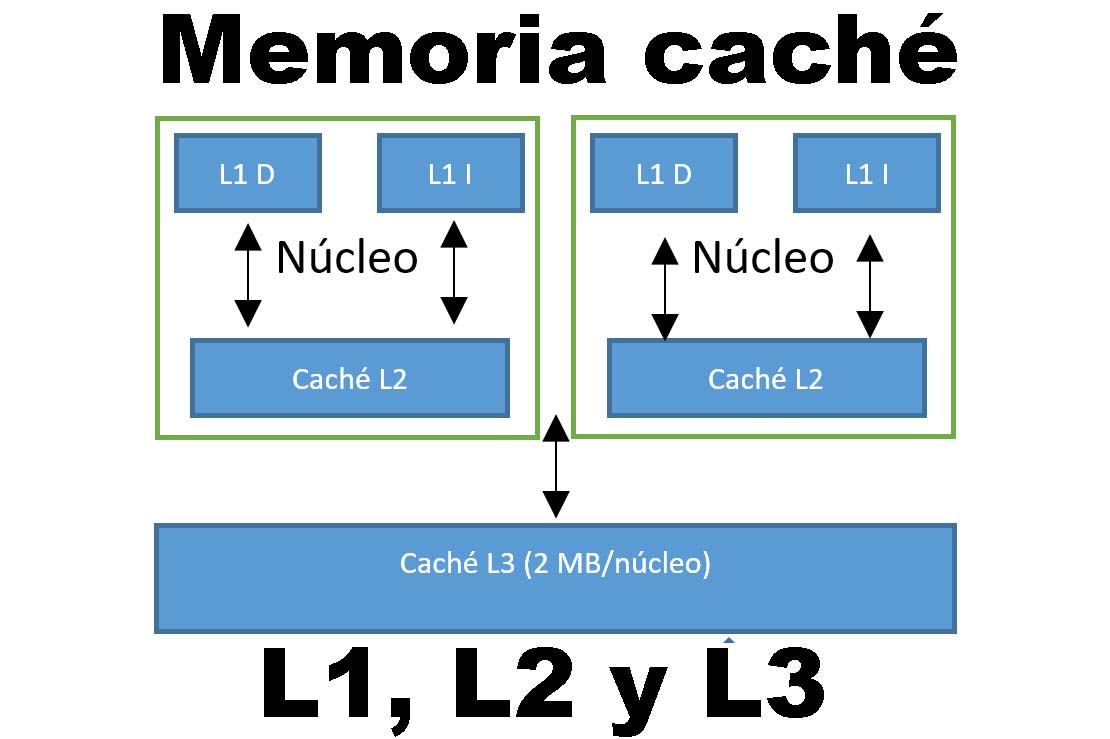
\includegraphics[width=6cm]{images/cache.jpg}
    \centering
    \label{fig:aleatory}
    \caption{Memoria caché L1 , L2 , L3}
    \end{figure}

La memoria caché se clasifica Desde L1 (teniendo un coste/bit alto) y descendiendo hasta L3 (coste/bit menor). Esta memoria está espacialmente más cerca del procesador y además presenta mayor velocidad de acceso que la memoria tipo RAM. Su función es facilitar el acceso de instrucciones 
 periódicas 
 para así disminuir la latencia que se experimenta al traer las instrucciones al procesador. Las instrucciones más usadas se almacenará en caché L1 y así hasta descender caché L3.
(su tamaño comúnmente se clasifica en Megabytes)

\section{Gestión de la memoria}


\section{Comparativa entre memorias}
 esta es la comparativa de las memorias

\section{Conclusión} 
conclusión del documento



\bibliographystyle{IEEEtran}
\bibliography{references}
\cite{rebollo}
\cite{figura1}
\end{document}
